\documentclass[11pt]{article}
\usepackage[utf8]{inputenc}
\usepackage[T1]{fontenc}
\usepackage{amsmath, amssymb}
\usepackage[margin=1in]{geometry}
\usepackage{xcolor}
\usepackage{listings}
\usepackage{graphicx}
\usepackage{booktabs}
\usepackage{enumitem}
\usepackage{hyperref}
\usepackage{epigraph}

\setlength{\epigraphwidth}{0.55\textwidth}
\renewcommand{\epigraphflush}{center}
\renewcommand{\epigraphrule}{0pt}

\lstset{
  language=Python,
  basicstyle=\ttfamily\small,
  keywordstyle=\color{blue!70!black},
  commentstyle=\color{gray!70},
  stringstyle=\color{green!40!black},
  showstringspaces=false,
  frame=single,
  breaklines=true,
  columns=fullflexible
}

\hypersetup{colorlinks=true, linkcolor=blue!60!black, urlcolor=blue!60!black}

% ----------------------------------------------------------------
\begin{document}
% ----------------------------------------------------------------

\epigraph{\itshape Come play my game}{``Breathe'' --- \textsc{The Prodigy} (1994)}

\begin{center}
  {\large\scshape University of Austin}\\[0.4cm]
  {\Large\bfseries Linear Algebra: Mathematics and Computation}\\[0.4cm]
  \hrulefill\\[0.4cm]
  {\large Lecture~1 $\cdot$ A First Look: Something Strange Is Happening}\\[0.2cm]
  {\normalsize Spring 2026}
\end{center}

\bigskip\noindent
\textit{You don't need to understand everything today.
That's the point.
Run the code, look at the pictures, notice what feels weird.
By the last lecture, every surprise here will feel obvious.}

\bigskip

% ================================================================
\section*{\S1 \quad A Game That Started It All}
% ================================================================

\noindent
In 1970, the mathematician John Conway invented a game played on an infinite grid of
square cells.
Each cell is either \textbf{alive} or \textbf{dead}.
Every tick, each cell looks at its eight neighbours and decides whether to
live or die according to a few simple counting rules.

\medskip\noindent
That's it.
No physics, no equations, no randomness.
Just a grid, and a rule.

\medskip\noindent
From this absurdly simple setup, something remarkable emerges: a tiny five-cell
pattern called the \textbf{glider}.
The glider moves — diagonally, one step every four ticks — forever, across
the infinite grid.

\begin{figure}[h]
  \centering
  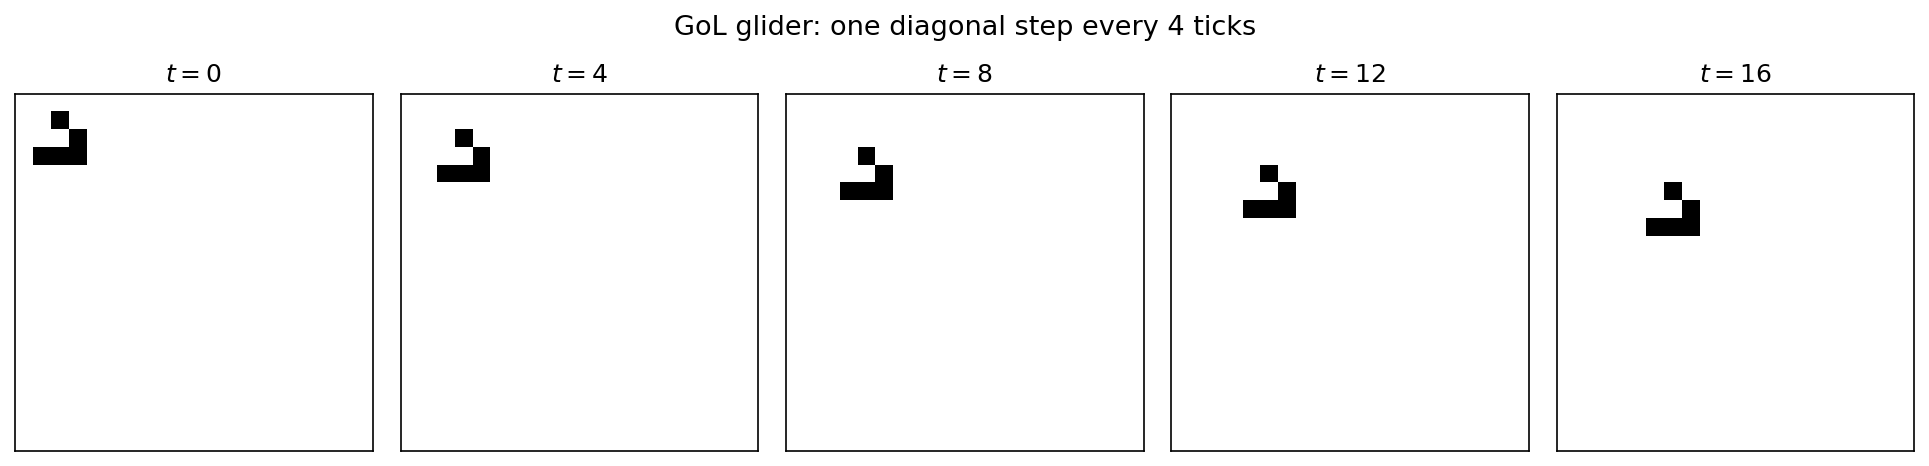
\includegraphics[width=0.92\textwidth]{../intro/fig_glider.png}
  \caption{The GoL glider at five snapshots, each four ticks apart.
           The pattern shifts one cell diagonally each time.}
\end{figure}

\medskip\noindent
Look at the glider's shape.
It is not symmetric: it has a leading edge pointing north-east and a trailing
edge to the south-west.
Each tick, the cells at the NE edge have just the right number of neighbours
to be born; the cells at the SW edge do not, and die.
The pattern shifts NE \emph{because its own shape is biased that way}.

\medskip\noindent
Here is the question that will drive this entire course:

\medskip
\begin{center}
\colorbox{yellow!25}{\parbox{0.82\textwidth}{
\centering\itshape
Fine — but why does the glider \emph{stay together}?\\[4pt]
Why doesn't it just break apart as it moves?\\[4pt]
There is something special about the diagonal direction that lets
coherent structures travel along it without dispersing.
}}
\end{center}

\medskip\noindent
We will answer this question completely.
But not today.

\bigskip

% ================================================================
\section*{\S2 \quad A Simpler Version}
% ================================================================

\noindent
Conway's Game of Life is \emph{nonlinear}: the rules involve counting
and comparing to thresholds.
Nonlinear systems are hard.
Let's replace GoL with something we can actually analyse.

\medskip\noindent
Instead of alive/dead, let each cell $(m, n)$ carry a real number
$u_{m,n}(t)$ — think of it as an \emph{activity level}.
And instead of the threshold rule, we use a plain \emph{linear} rule:

\bigskip
\begin{equation}
  \boxed{u_{m,n}(t+1) \;=\; 1.2\cdot u_{m+1,\,n+1}(t) \;+\; 0.8\cdot u_{m-1,\,n-1}(t)}
\end{equation}
\bigskip

\noindent
In plain English: \textit{``Next activity = 1.2 $\times$ north-east neighbour
                           + 0.8 $\times$ south-west neighbour.''}

\medskip\noindent
Notice: this rule only ever talks to the NE and SW neighbours.
It completely ignores NW and SE.
The weights are not arbitrary.
In GoL, a dead cell is \emph{born} when it has exactly \textbf{3}~alive
neighbours, and an alive cell \emph{survives} when it has at least \textbf{2}.
The glider's NE cells are the ones being born (the 3-neighbour condition);
its SW cells are the ones dying.
We encode that asymmetry directly: NE gets weight proportional to~3, SW
proportional to~2, scaled so the two weights sum to~2:
\[
  p \;=\; 2 \cdot \tfrac{3}{5} = 1.2, \qquad
  q \;=\; 2 \cdot \tfrac{2}{5} = 0.8.
\]
This is not a rigorous derivation — it is an analogy.
But it is the right analogy.

\medskip\noindent
What happens when you run it?
Let's find out.

\bigskip

% ================================================================
\section*{\S3 \quad Let's Experiment}
% ================================================================

\subsection*{Experiment 1 — drop a single blip}

\noindent
Start with a 64$\times$64 grid, all zeros except one cell in the centre set to~1.
Run the rule for 20 steps.

\begin{lstlisting}
import numpy as np
import matplotlib.pyplot as plt

N = 64
p, q = 1.2, 0.8

def step(u):
    # u[m,n] gets p times its NE neighbour and q times its SW neighbour
    return p * np.roll(np.roll(u, -1, axis=0), -1, axis=1) \
         + q * np.roll(np.roll(u, +1, axis=0), +1, axis=1)

# Start with a single active cell at the centre
u = np.zeros((N, N))
u[N//2, N//2] = 1.0

frames = [u.copy()]
for _ in range(20):
    u = step(u)
    frames.append(u.copy())
\end{lstlisting}

\begin{figure}[h]
  \centering
  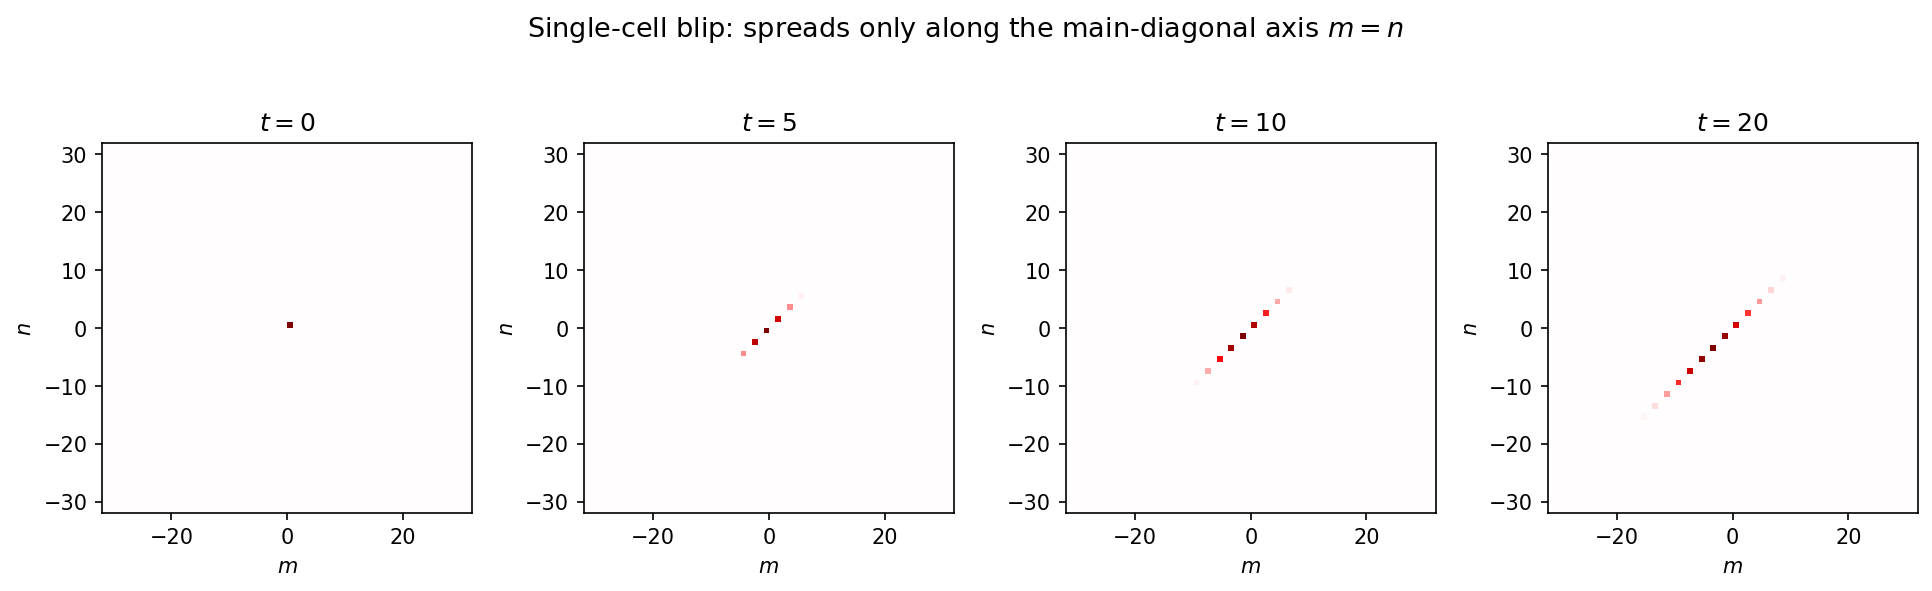
\includegraphics[width=0.92\textwidth]{../intro/fig_blip.png}
  \caption{A single blip at the centre, evolved for 20 steps.
           Each frame is 4 ticks later.}
\end{figure}

\noindent
The signal spreads only along \textbf{one diagonal} — north-east / south-west.
The other diagonal carries nothing.
No mystery: the rule only couples NE and SW neighbours, so information can only
travel that way.

\subsection*{Experiment 2 — how fast does it grow?}

\begin{lstlisting}
energies = [np.sum(np.abs(f)) for f in frames]
for t, e in enumerate(energies):
    print(f"t={t:2d}   total activity = {e:.4f}")
\end{lstlisting}

\noindent
Each step the total activity \textbf{doubles}.
Always.
Every single step, right from the start.
Yet neither 1.2 nor 0.8 equals~2.
Where does 2 come from?

\medskip\noindent
(Spoiler: $1.2 + 0.8 = 2$.
But \textit{why} is it the sum?
That's a linear algebra story.)

\subsection*{Experiment 3 — does direction matter?}

\noindent
Instead of a single blip, seed the grid with a wave running along each
diagonal — first the \emph{anti-diagonal} (NW--SE), then the \emph{main diagonal}
(NE--SW) — and watch what happens.

\begin{figure}[h]
  \centering
  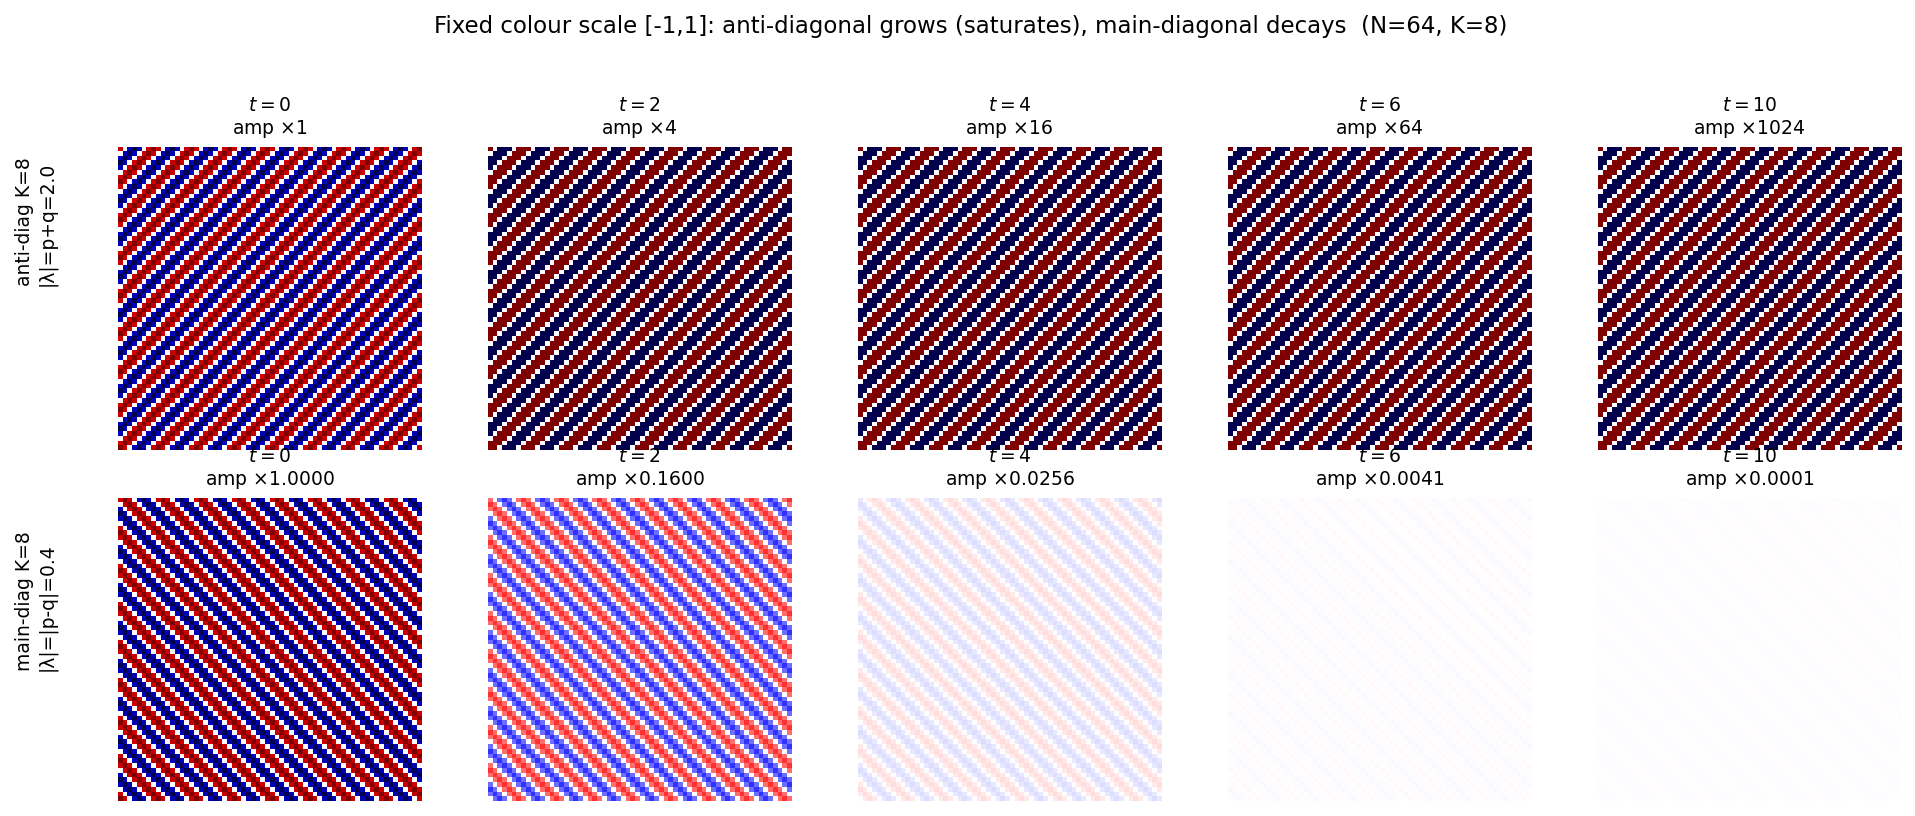
\includegraphics[width=0.92\textwidth]{../intro/fig_stripes.png}
  \caption{Top row: wave along the anti-diagonal.
           Bottom row: wave along the main diagonal.
           The anti-diagonal wave stays a perfect stripe forever
           (just $1024\times$ bigger after 10 steps).
           The main-diagonal wave at this wavelength fades to nothing in 10 steps.}
\end{figure}

\noindent
So direction matters — a lot.
Every anti-diagonal wave grows at rate~2, regardless of its wavelength.
Main-diagonal waves grow or shrink depending on their wavelength.

\medskip\noindent
That last part is the key.
When different wavelengths grow at \emph{different} rates, a pattern made of
several wavelengths falls apart: the fast components outrun the slow ones.
The anti-diagonal direction is special precisely because all wavelengths grow at
the \emph{same} rate~2 — a pattern moving in that direction stays together.

\bigskip

% ================================================================
\section*{\S4 \quad The Full Picture}
% ================================================================

\noindent
Here is a map of every possible wave direction on the grid, coloured by
how fast it grows or shrinks under one step of the rule.

\begin{figure}[h]
  \centering
  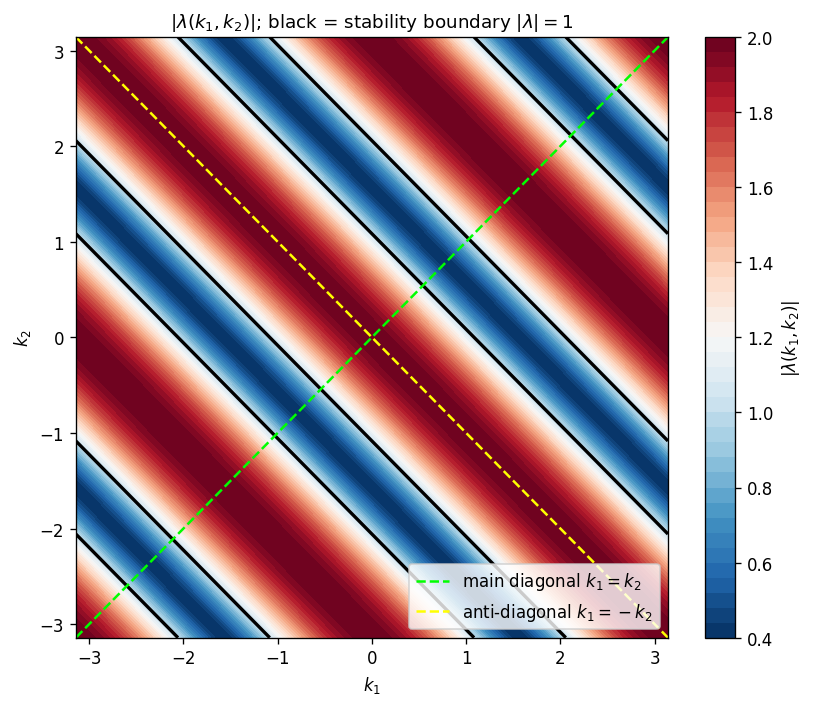
\includegraphics[width=0.72\textwidth]{../intro/fig_amplification_map.png}
  \caption{Growth rate $|\lambda(k_1, k_2)|$ for every possible wave direction
           in the grid.
           Black curve = boundary between growing and decaying.
           The anti-diagonal axis (yellow dashes) sits entirely in the
           `growing' region, always at exactly~2.
           The main-diagonal axis (green dashes) crosses the boundary.}
\end{figure}

\noindent
Each point is a wave direction. Red = growing, blue = decaying.
The yellow dashed line (anti-diagonal) sits entirely in the red zone — every
wave in that direction grows at exactly~2.
The green dashed line (main diagonal) cuts across: some wavelengths grow, some
shrink.

\medskip\noindent
By the end of this course you will be able to derive this picture from scratch
using two ideas: \textbf{eigenvectors} and the \textbf{Fourier transform}.
For now, just look at it.

\bigskip

% ================================================================
\section*{\S5 \quad What This Course Will Teach You}
% ================================================================

\noindent
Here is what the next few months are about, in plain terms.

\begin{enumerate}[leftmargin=1.5em, itemsep=0.6em]

  \item \textbf{Vectors and linear maps.}
        The rule $u \mapsto Tu$ is a \emph{linear map}.
        Linear maps are the centrepiece of the course.
        We will spend a long time understanding what they can and cannot do.

  \item \textbf{Eigenvalues and eigenvectors.}
        The waves in \S3 are \emph{eigenvectors} of $T$.
        Their growth rates are \emph{eigenvalues}.
        Once you know them, you can predict everything.

  \item \textbf{Change of basis.}
        Switching to the `wave basis' (the Fourier basis) turns $T$ into a
        simple diagonal map — multiply each component by its eigenvalue.
        This is why the FFT is fast.

  \item \textbf{Stability.}
        A system is stable when all eigenvalues have magnitude $\leq 1$.
        The black curve in \S4 is exactly the set of unstable modes.

\end{enumerate}

\bigskip\noindent
\begin{center}
\colorbox{gray!10}{\parbox{0.88\textwidth}{
\itshape
Here is the full story, in plain terms.\\[6pt]
The GoL glider moves NE because its shape has a NE bias: the leading edge
is born, the trailing edge dies.
Our linear model copies that bias directly — NE neighbour gets weight~1.2,
SW gets~0.8.\\[6pt]
The glider \emph{stays coherent} as it moves because the diagonal direction
has a special property: every wave pattern along it grows at the same rate.
Patterns made of many wavelengths can travel together without falling apart.
In all other directions, different wavelengths grow at different rates and
any coherent structure disperses.\\[6pt]
Our linear model shows exactly this.
And the same mechanism is at work in GoL.\\[6pt]
\textbf{By the end of this course, you will be able to prove all of this from scratch.}
}}
\end{center}

\bigskip

\end{document}
